%------------------------
% Anschreiben – Robotics and Computer Vision Engineer
% Bewerbung bei: metamorphosis GmbH
% Verfasser: Shrikar Nakhye
%------------------------

\documentclass[a4paper,10pt]{article}

\usepackage{latexsym}
\usepackage[empty]{fullpage}
\usepackage{titlesec}
\usepackage{marvosym}
\usepackage[usenames,dvipsnames]{color}
\usepackage{verbatim}
\usepackage{enumitem}
\usepackage[hidelinks]{hyperref}
\usepackage{fancyhdr}
\usepackage{tabularx}
\usepackage{graphicx}

\newlength{\origtextwidth}

\pagestyle{fancy}
\fancyhf{} % clear all header and footer fields
\fancyfoot{}
\renewcommand{\headrulewidth}{0pt}
\renewcommand{\footrulewidth}{0pt}

% Adjust margins & Fix footskip warning
\addtolength{\oddsidemargin}{-0.530in}
\addtolength{\evensidemargin}{-0.375in}
\addtolength{\textwidth}{1in}
\addtolength{\topmargin}{-.60in}
\addtolength{\textheight}{1.5in}
\setlength{\footskip}{3.60004pt}

\urlstyle{rm}

\raggedbottom
\raggedright
\setlength{\tabcolsep}{0in}

\begin{document}

%----------HEADING-----------------
\setlength{\origtextwidth}{\textwidth}
\definecolor{headerbg}{RGB}{242, 244, 247}
\vspace*{-\dimexpr\topmargin+1in\relax}
\noindent
\makebox[\origtextwidth][c]{%
  \colorbox{headerbg}{%
    \begin{minipage}{\paperwidth}
      \vspace*{16pt}
      \hspace{\dimexpr\oddsidemargin+1in\relax}%
      \begin{minipage}[c]{0.72\origtextwidth}
          \raggedright
          {\Huge \textbf{Shrikar Nakhye}} \\[6pt]
          \small
          Anschrift: Bonn, Deutschland \\
          E-Mail: \href{mailto:nakhyeshrikar@icloud.com}{nakhyeshrikar@icloud.com} \\
          Geburtsdatum: 30. August 2000 \\[6pt]
          \raisebox{-2pt}{
\includegraphics[height=10pt]{images/LinkedIn.png}}\ \href{https://www.linkedin.com/in/shrikar-nakhye-053262188/}{LinkedIn} \quad
          \raisebox{-2pt}{
\includegraphics[height=10pt]{images/github.png}}\ \href{https://github.com/ItsShriks}{GitHub} \quad
          \raisebox{-2pt}{
\includegraphics[height=10pt]{images/Google_Scholar.png}}\ \href{https://scholar.google.com/citations?user=-kVcoO8AAAAJ&hl=en}{Google Scholar}
      \end{minipage}%
      \hfill
      \begin{minipage}[c]{0.20\origtextwidth}
          \raggedleft
          {\setlength{\fboxsep}{0pt}\fbox{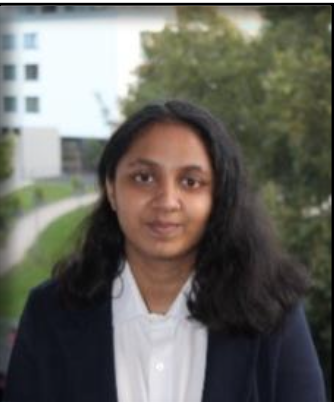
\includegraphics[width=2.5cm,height=3.3cm,keepaspectratio]{images/Self_Pic.jpg}}}
      \end{minipage}%
      \hspace{\dimexpr\oddsidemargin+1in\relax}%
      \vspace{8pt}
    \end{minipage}%
  }%
}

\vspace{12pt}
\hspace{0.015\textwidth}
\begin{minipage}{0.97\textwidth}

\vspace{6pt}

\textbf{An:} \\
Deutsches Zentrum für Luft- und Raumfahrt e. V. (DLR) \\
Institut für den Schutz terrestrischer Infrastrukturen \\
z. Hd. Dr. Tobias Koch \\
Rathausallee 12 \\
53757 Sankt Augustin \\

\vspace{6pt}

\textbf{Betreff: Bewerbung für eine Masterarbeit – Drohnen-Tracking (Kennziffer 5841)}

\vspace{6pt}

Sehr geehrter Herr Dr. Koch,

\vspace{3pt}

mit großem Interesse bewerbe ich mich um die ausgeschriebene Masterarbeit im Bereich ``Drohnen-Tracking'' (Kennziffer 5841) an Ihrem Institut für den Schutz terrestrischer Infrastrukturen. Die Mission des DLR, kritische Infrastrukturen durch innovative Sicherheitsarchitekturen resilienter zu machen, und insbesondere der Einsatz kamerabasierter Detektion und Verfolgung zur Abwehr ziviler Bedrohungen faszinieren mich sehr. Als immatrikulierter Masterstudent in Autonomous Systems an der Hochschule Bonn-Rhein-Sieg bringe ich fundierte Vorkenntnisse in Computer Vision, Deep Learning sowie praktischer Algorithmen-Evaluation mit und möchte meine Abschlussarbeit diesem zukunftsweisenden Thema widmen.

\vspace{3pt}

Durch meine bisherigen akademischen und beruflichen Stationen bringe ich ein optimal passendes Profil für die anspruchsvollen Aufgaben bei der DLR-Masterarbeit mit:

\vspace{2pt}

\begin{itemize}[leftmargin=*, itemsep=2pt, topsep=2pt]

    \item \textbf{Echtzeit-Tracking unter Okklusionen}: Als Kernmitglied des Robotik-Teams \textit{b-it bots @Home} habe ich unter ROS 2 ein modulares \textit{Detect-then-Track}-Framework zur Personenverfolgung implementiert. Durch die Integration von OpenCV und MediaPipe konnte ich eine Tracking-Erfolgsquote von 95\% erzielen, selbst unter schwierigen Bedingungen wie temporären Okklusionen. Dies qualifiziert mich direkt für die Evaluation und Stabilisierung von Tracking-by-Detection-Verfahren bei temporären Detektionsausfällen.

    \item \textbf{Verarbeitung von Drohnen-Datensätzen}: In meiner Rolle als Wissenschaftliche Hilfskraft an der H-BRS war ich für das Design und die CUDA-Beschleunigung von 3D-Segmentierungsalgorithmen zur Echtzeitverarbeitung hochauflösender Drohnendatensätze verantwortlich. Dabei konnte ich die Verarbeitungsgenauigkeit um 15\% steigern. Ich bin daher bestens vertraut mit den Herausforderungen von Luftbilddaten sowie dem Handling großer Datensätze.

    \item \textbf{Deep Learning und PyTorch}: Ich verfüge über fundierte Programmierkenntnisse in Python und weitreichende praktische Erfahrung im Training, der Evaluation und der Integration von Deep-Learning-Wahrnehmungsmodellen (insbesondere YOLO/PyTorch). Dies ermöglicht mir eine schnelle Einarbeitung und die nahtlose Implementierung von transformerbasierten Tracking-Architekturen.

    \item \textbf{Wissenschaftliche Arbeitsweise und Dokumentation}: Mein solides mathematisch-technisches Fundament spiegelt sich auch in meinen bisherigen Beiträgen wider: Ich habe bereits vier wissenschaftliche Arbeiten (u. a. bei der IEEE) veröffentlicht. Ich bin gewohnt, methodisch vorzugehen, Ergebnisse anhand etablierter Metriken systematisch zu evaluieren und diese präzise schriftlich auszuarbeiten.

\end{itemize}

\vspace{3pt}

Als immatrikulierter Masterstudent an der nahegelegenen H-BRS kann ich die Masterarbeit ab sofort beginnen und freue mich darauf, mich für die verbleibenden 6 Monate intensiv in Ihr Team einzubringen. Ich spreche fließend Englisch (C2) sowie Deutsch auf B2-Niveau, was mir eine reibungslose Kommunikation im interdisziplinären Forschungsumfeld des DLR ermöglicht.

\vspace{3pt}

Ich freue mich sehr über die Gelegenheit, Ihnen meine Motivation und Eignung in einem persönlichen Gespräch näher vorzustellen.

\vspace{10pt}

Mit freundlichen Grüßen,

\vspace{8pt}
Shrikar Nakhye

\end{minipage}

\end{document}

